\begin{figure}[htbp]
 \centering
 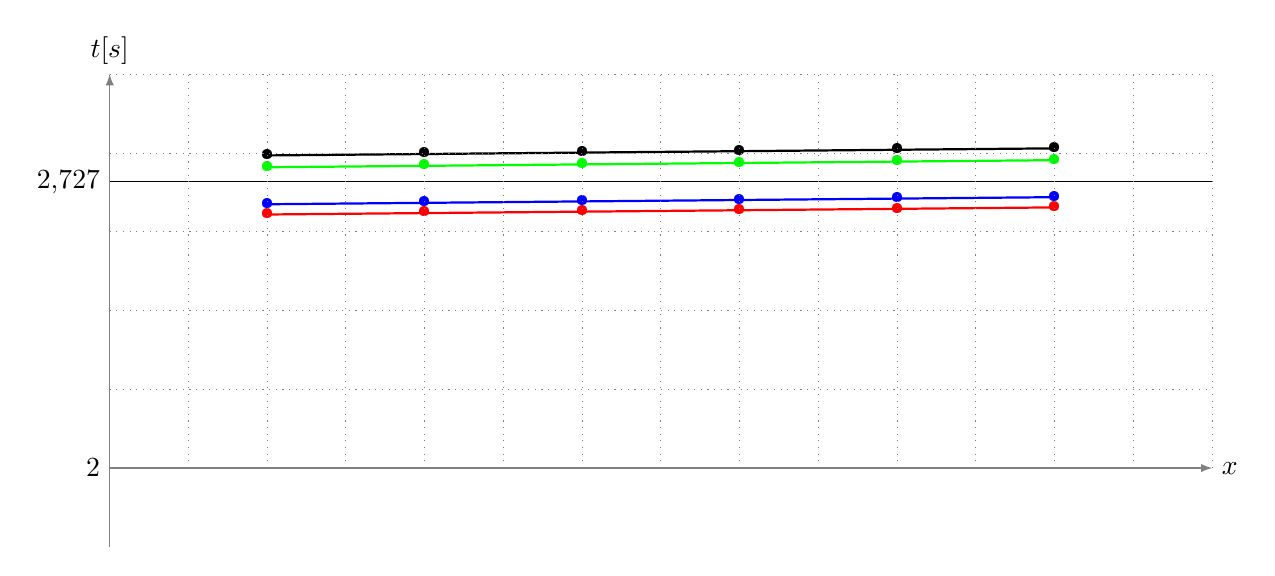
\begin{tikzpicture}[x=2cm,y=5cm]


 \draw[-latex, thin, draw=gray] (0,2)--(7,2) node [right] {$x$}; % l'axe des abscisses
 \draw[-latex, thin, draw=gray] (0,1.8)--(0,3) node [above] {$t[s]$}; % l'axe des ordonnées
 \draw (0,2) node[left] {2};
 \draw[] (0,2.727)--(7,2.727) node[left=14cm] {2,727}; 

%Pierwszy pomiar   
	\node at (1, 2.794) {\textbullet};
	\node at (2, 2.798) {\textbullet};
	\node at (3, 2.802) {\textbullet};
	\node at (4, 2.804) {\textbullet};
	\node at (5, 2.808) {\textbullet};
	\node at (6, 2.812) {\textbullet};		
	
	\draw[thick] (1, 2.794)--(6, 2.812);
	
%Drugi pomiar			
	\node[red] at (1, 2.644) {\textbullet};
	\node[red] at (2, 2.648) {\textbullet};
	\node[red] at (3, 2.652) {\textbullet};
	\node[red] at (4, 2.654) {\textbullet};
	\node[red] at (5, 2.658) {\textbullet};
	\node[red] at (6, 2.662) {\textbullet};
	
    \draw[thick,red] (1, 2.644)--(6, 2.662);
    
%Trzeci pomiar
	\node[blue] at (1, 2.670) {\textbullet};
	\node[blue] at (2, 2.674) {\textbullet};
	\node[blue] at (3, 2.678) {\textbullet};
	\node[blue] at (4, 2.680) {\textbullet};
	\node[blue] at (5, 2.684) {\textbullet};
	\node[blue] at (6, 2.688) {\textbullet};
	
    \draw[thick,blue] (1, 2.670)--(6, 2.688);
        
%Czwarty pomiar    
	\node[green] at (1, 2.764) {\textbullet};
	\node[green] at (2, 2.768) {\textbullet};
	\node[green] at (3, 2.772) {\textbullet};
	\node[green] at (4, 2.774) {\textbullet};
	\node[green] at (5, 2.778) {\textbullet};
	\node[green] at (6, 2.782) {\textbullet};
	
    \draw[thick,green] (1, 2.764)--(6, 2.782);
     
% to ensure that the points are being properly centered:
\draw [dotted, gray] (0,2) grid (7,3);

\end{tikzpicture}
\caption{Pomiary czasu ponownego podłączenia oraz obliczona wartość średnia}
\label{badania:wykres:stabilizacja_wyspa}
\end{figure}